\clearpage
\section*{Problem 3}
\begin{enumerate}[a)]
    \item The Five Requirements
    \begin{enumerate}[i.]
        \item BELL = ER \&\& !DSBF
        \item BELL = ER \&\& !DC
        \item BELL = DSBF \&\& !ER \&\& DC
        \item DLA = !DOS \&\& !KIC
        \item BA = BP \&\& CM
    \end{enumerate}
    \item Truth Table\\
    \begin{tabular}{|c|c|c|c|c|c|c|c|c|c|c|c}
        \hline
        DOS & DSBF & ER & DC & KIC & DLC & BP & CM & BELL & DLA & BA \\
        \hline
        X & 0 & 1 & X & X & X & X & X & 1 & X & X\\
        \hline
        X & X & 1 & 0 & X & X & X & X & 1 & X & X\\
        \hline
        X & 1 & 0 & 1 & X & X & X & X & 0 & X & X\\
        \hline
        0 & X & 1 & X & X & X & X & X & X & 1 & X\\
        \hline
        X & X & X & X & X & X & 1 & 1 & X & X & 1\\
        \hline
    \end{tabular}
    
    \item Code
    
    \begin{figure}[!ht]
        \centering
        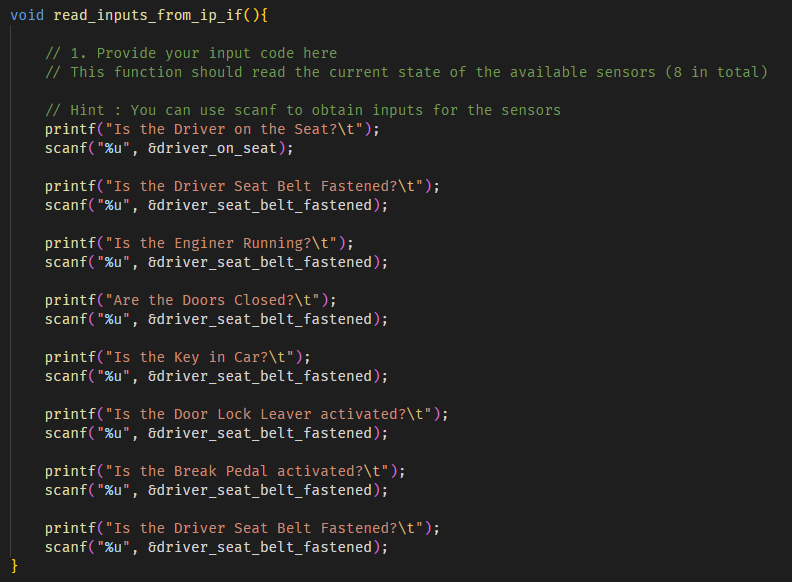
\includegraphics[width=0.5\textwidth]{Images/3a Code Read.png}
        \caption{Read Inputs}
    \end{figure}
    
    \begin{figure}[!ht]
        \centering
        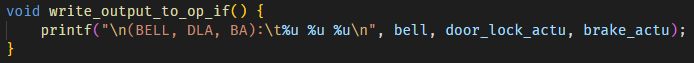
\includegraphics[width=0.9\textwidth]{Images/3a Code Write.png}
        \caption{Write Output}
    \end{figure}
    
    \begin{figure}[!ht]
        \centering
        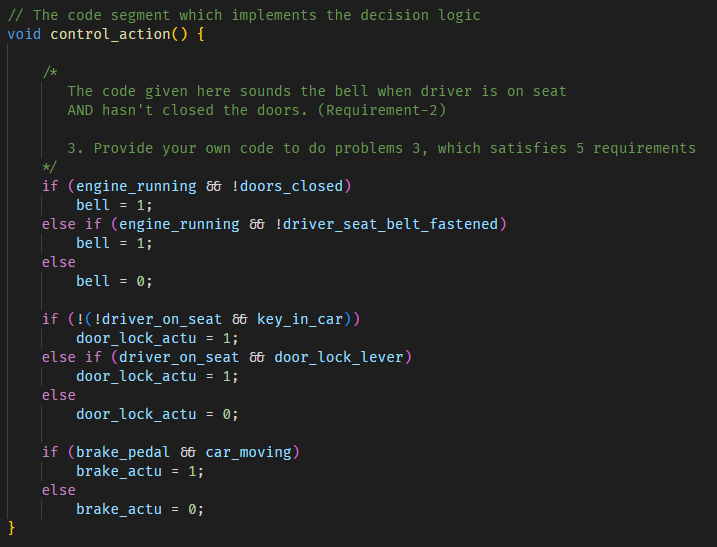
\includegraphics[width=0.9\textwidth]{Images/3a Code Logic.png}
        \caption{Logic}
    \end{figure}

    \begin{figure}[!htt]
        \centering
        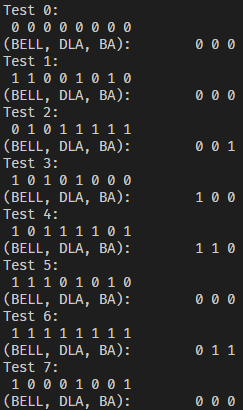
\includegraphics{Images/3d Output.png}
        \caption{Output}
    \end{figure}
\end{enumerate}